\documentclass[12pt,a4paper]{article}
\usepackage[T1]{fontenc}
\usepackage[utf8]{inputenc}
\usepackage{newtxtext,newtxmath}
\usepackage[margin=1in]{geometry}
\usepackage{setspace}
\usepackage{amsmath}
\usepackage{booktabs}
\usepackage{graphicx}
\usepackage{caption}
\usepackage{array}
\usepackage{tabularx}
\usepackage{ragged2e}
\usepackage[hidelinks]{hyperref}

\captionsetup[table]{labelsep=period,justification=raggedright,
  singlelinecheck=false,font={it},labelfont={it}}
\captionsetup[figure]{labelsep=period,justification=raggedright,
  singlelinecheck=false,font={it},labelfont={it}}

\setlength{\parindent}{0pt}
\setlength{\parskip}{6pt}
\doublespacing

\newcommand{\mainhead}[1]{%
  \par\vspace{10pt}\noindent\textbf{\MakeUppercase{#1}}\par\vspace{2pt}}
\newcommand{\subhead}[1]{%
  \par\vspace{6pt}\noindent\textbf{\textit{#1}}\par\vspace{1pt}}

\begin{document}


\begin{center}\textbf{\large From Statistical Evidence to Decision Value: Six Deployment Constraints on an Institutional Flow Dataset}\end{center}

\mainhead{ABSTRACT}

\textbf{Purpose.} This study asked how far an alternative dataset carries once its statistical content is settled, under the constraints a deployed use would face.

\textbf{Design/Methodology/Approach.} A fourteen-year record of foreign institutional flow in Indian equities, covering 25.2 million trades, was applied at seven points in a modelling stack: a volatility regression, a real-time filtered regime model with a hazard layer, stock-day and market-level predictive densities, a gradient-boosted feature block, and a long-short book. Each faced six ascending constraints: existence, era stability on a frozen holdout, availability at the decision lag, competition against the deployed baseline, detectability in the consuming metric, and execution cost. Each application was evaluated against a threshold fixed before its own result was generated, and an outside predictor passed through the same machinery as a control.

\textbf{Findings.} None failed at the first two constraints. Six of the seven then failed, at four different constraints. One survived, aggregated to market level at a measured two-day reporting lag against a baseline that did not contain it, though its margin is slim once the search is priced. The control failed at the same constraint as two of the seven, consistent with the difficulty arising at the evaluation-to-deployment transition rather than in the data.

\textbf{Practical Implications.} Different implementations of one record met different binding constraints. Practitioners should establish the deployable lag, competing baseline and breakeven cost before establishing significance.

\textbf{Originality/Value.} Existing work imposes one constraint across many predictors; this study imposed six, in sequence, across one dataset.

\textbf{Keywords:} alternative data, institutional flow, forecast evaluation, transaction costs, replication, risk models

\textbf{JEL Classification:} G12, G14, G17, C52, C58

\mainhead{INTRODUCTION}

Most published return predictors do not survive re-testing. Hou et al. (2020) re-examined 452 anomalies and found that 65\% failed a conventional significance hurdle once microcaps were handled properly, rising to 82\% under a multiple-testing threshold. Jensen et al. (2023) reached a more optimistic verdict on a broader factor set, and the disagreement between the two remains open. What neither settles is what becomes of the findings that do pass.

This study addresses that remainder. It takes one dataset whose statistical content is never in question, and asks how far that content carries once the tests stop being statistical.

The object of study is the data, not the models built on it. A cross-sectional regression, a regime model, a density engine and a book of strategies appear below, and none is offered as a contribution. Each imposes one kind of real-world constraint on the same record. When an ablation shows that a regime model's conditioning adds nothing to a risk density, that is a measurement about the flow data, not a verdict on hidden Markov models.

Six constraints organise the analysis, and a result must clear each to reach the next: existence under conventional inference, era stability on a frozen era the design never touched, availability when the decision must be taken, competition against the baseline the application would be deployed against, detectability in the metric the decision consumes, and execution against the cost of capture. The ordering follows institutional reality rather than statistical severity: the first two concern the sample, the remaining four concern deployment.

Because the sequence is ordered, the level at which an application stops is a complete statement of how far the data carried in that use. Read across applications, the binding constraint varies with the implementation rather than with the market. The same record, aggregated differently and scored against a different baseline, meets a different binding constraint.

The study contributes three things: a boundary rather than a verdict, since one application survives and the result maps where the record's value stops; evidence that different implementations of one record meet different binding constraints, since six fail at four levels; and a provenance protocol binding every reported figure to the artifact that produced it, its digest, and an extractor that reads the value back out. The design cannot show that the ordering generalises, and no such claim is made.

\mainhead{REVIEW OF LITERATURE}

\subhead{Replication and the Credibility of Published Findings}

Hou et al. (2020) re-examined 452 anomalies and reported that 65\% failed a conventional significance hurdle once microcaps were handled through appropriate breakpoints and value weighting, rising to 82\% under a multiple-testing threshold. Jensen et al. (2023) reached the opposite conclusion on a broader factor set, finding most factors replicate once modelled jointly; the disagreement turns on the criterion applied rather than on the data. Bowles et al. (2024) showed that when an anomaly's returns occur, relative to its discovery date, changes what the evidence supports; Chai et al. (2026) documented how often replication fails in practice; and Chopra et al. (2023) measured the publication penalty on null findings, which explains why studies reporting what did not survive remain uncommon. Two features bear on the present study: this literature asks whether an effect exists, and evaluates many predictors under a single criterion. Both leave open what becomes of the findings that pass.

\subhead{Constraints Between Statistical Significance and Practical Use}

A second strand imposes a single friction across many candidate findings. Muravyev et al. (2025) applied short-sale costs to 162 anomalies, turning an average long-short return of 0.14\% per month before borrow fees into −0.01\% after. Kaplanski (2023) examined the cost of slow trading as competitors race to exploit a documented effect, and Pénasse (2022) modelled the decay of an edge after discovery. Machine-learning work has begun to price design choices rather than predictors: Bagnara (2024) identified transaction costs and research design as the recurring weak points, Sak et al. (2024) pruned the factor zoo under a portfolio criterion and found most surviving factors carry risk prices indistinguishable from zero, and Azevedo et al. (2023) and Li et al. (2024) tested anomalies internationally and in Chinese A-shares. Each varies the predictor set while holding the evaluation criterion fixed.

\subhead{Evaluating Forecasts, Densities, and Backtests}

The forecast-evaluation literature supplies the instruments a deployment test requires. Allen et al. (2025) set out tail calibration and Waghmare and Ziegel (2026) surveyed proper scoring rules, both bearing on the choice of metric when a claim concerns the tail rather than the centre. Arnold et al. (2024) decomposed the continuous ranked probability score, allowing a score difference to be attributed. Gonçalves et al. (2025) established predictive-ability inference under data revision, and Arian et al. (2024) showed how sharply false discovery depends on the set of competing models retained.

\subhead{Alternative Data and Its Valuation}

Coyle and Manley (2024) reviewed methods for valuing data as an asset and Sun et al. (2024) surveyed alternative data in finance; neither offers a worked case in which one dataset is carried through successive deployment constraints. On the instruments used below, Ghachem and Ersan (2025) advanced estimation of informed-trading models and Ding et al. (2025) applied regime-switching models to realised volatility across eight markets.

\subhead{Foreign Institutional Flow in the Indian Market}

The most directly relevant recent work concerns whether foreign trades in this market carry information. Raizada and Nawn (2025) found positive-feedback trading consistent with an informational disadvantage rather than an advantage; Thapa et al. (2026) showed how policy uncertainty shapes foreign institutional trading; Dey et al. (2024) examined how institutional investors here respond to risk, return and volatility; and Maheshwari and Naik (2026) documented the shift from foreign to domestic institutional dominance. This literature works almost entirely from aggregate or holdings-level data, because transaction-level records with participant attribution rarely leave depositories.

\subhead{Research Gap}

Three gaps follow. The replication literature establishes whether effects exist and stops there, leaving the surviving minority undocumented under deployment constraints. The friction literature imposes one constraint across many predictors, which cannot reveal whether the binding constraint varies across uses of the same information, because the constraint is fixed by design. And the alternative-data literature establishes that valuation methods exist without applying them to one dataset through an ordered sequence of realistic constraints.

\subhead{Objectives of the Study}

The study pursued three objectives, each expressed as a question the design can answer.

RQ1. Holding the data constant and varying the use, how far does a transaction-level record of foreign institutional flow carry at each of several points in a modelling stack?

RQ2. For each application, at which constraint does it stop, and do different implementations of the same record meet different binding constraints?

RQ3. Is the observed attrition peculiar to this record, or does a predictor drawn from outside the dataset attrite in the same way under identical machinery?

RQ1 is answered by the attrition in Figure 2; RQ2 by the spread of failures across constraints and, most directly, by the controlled pair in Table 2, where one predictor passes or fails according to the baseline it is scored against; RQ3 by the external control.

\mainhead{METHODOLOGY}

\subhead{The Record and Its Governing Constraint}

The object of study is a transaction-level record of foreign institutional activity in Indian equities, from depository settlement data. It covers 1 January 2011 to 31 March 2025 and 25,155,785 trades across 5,960 instrument identifiers, each carrying a date, an instrument, a masked participant identifier, a side and a traded value. Published data for this market is a daily aggregate; this record resolves to the instrument, day and participant, permitting statistics about the composition of flow that aggregate reporting cannot support.

Masked participant identifiers appear persistent and are not. The persistence statistic is computed on a control population whose real-world persistence is known independently: brokers and clearing members here number in the hundreds, yet over a 171-month span present as 22,262 identifiers with a median lifetime of one month. Masked participant identifiers behave identically, at 363,663 identifiers and the same median. Since the control cannot have that turnover, identifiers are re-minted monthly, so every entity statistic below is within-day.

Returns come from exchange settlement prices, with corporate-action factors verified against observed price ratios and a guard nulling any post-adjustment daily return above 50\%. Instrument identity is resolved through a point-in-time map with issuer-bounded closure. The modelling universe is 1,028 instruments over 802,806 instrument-days, by rule: an instrument-day enters if the record shows at least five trades in that instrument that day, and an instrument enters an era if it accumulates sixty such days within that era. The second condition is evaluated on the era total and then applied to the whole of that instrument's era, so an instrument reaching its sixtieth qualifying day late in an era keeps its earlier days. That is forward-looking within an era, and the exposure is bounded: a strictly causal rule would exclude the first fifty-nine qualifying days of each instrument-era, 10.8\% of instrument-days, without changing which instruments enter an era. Selection is on trading activity, not on returns, and it carries no survivorship across the split.

\subhead{Frozen Split and Missing Data}

Parameters, thresholds and specifications are fixed on data through 30 April 2021; the test era begins 1 July 2021. The intervening two months are absent at source, and the gap doubles as an embargo across a structural break. The eras are not a repeat sample: training covers 618 instruments across 508,563 instrument-days, test 851 across 294,243, and only 441 instruments appear in both. Three further months carry a wholly null direction flag, 3.004\% of trades, falling entirely within the test era; they are excluded, never imputed.

Figure 1 sets out the design. Parameters are sealed into dated vintages, each fitted on data preceding its own date and applied forward without restatement, so no figure reported for a given day uses information unavailable that day.

\begin{figure}[htbp]
\centering
\caption{Frozen Split, Embargo, and the Walk-Forward Vintage Design}
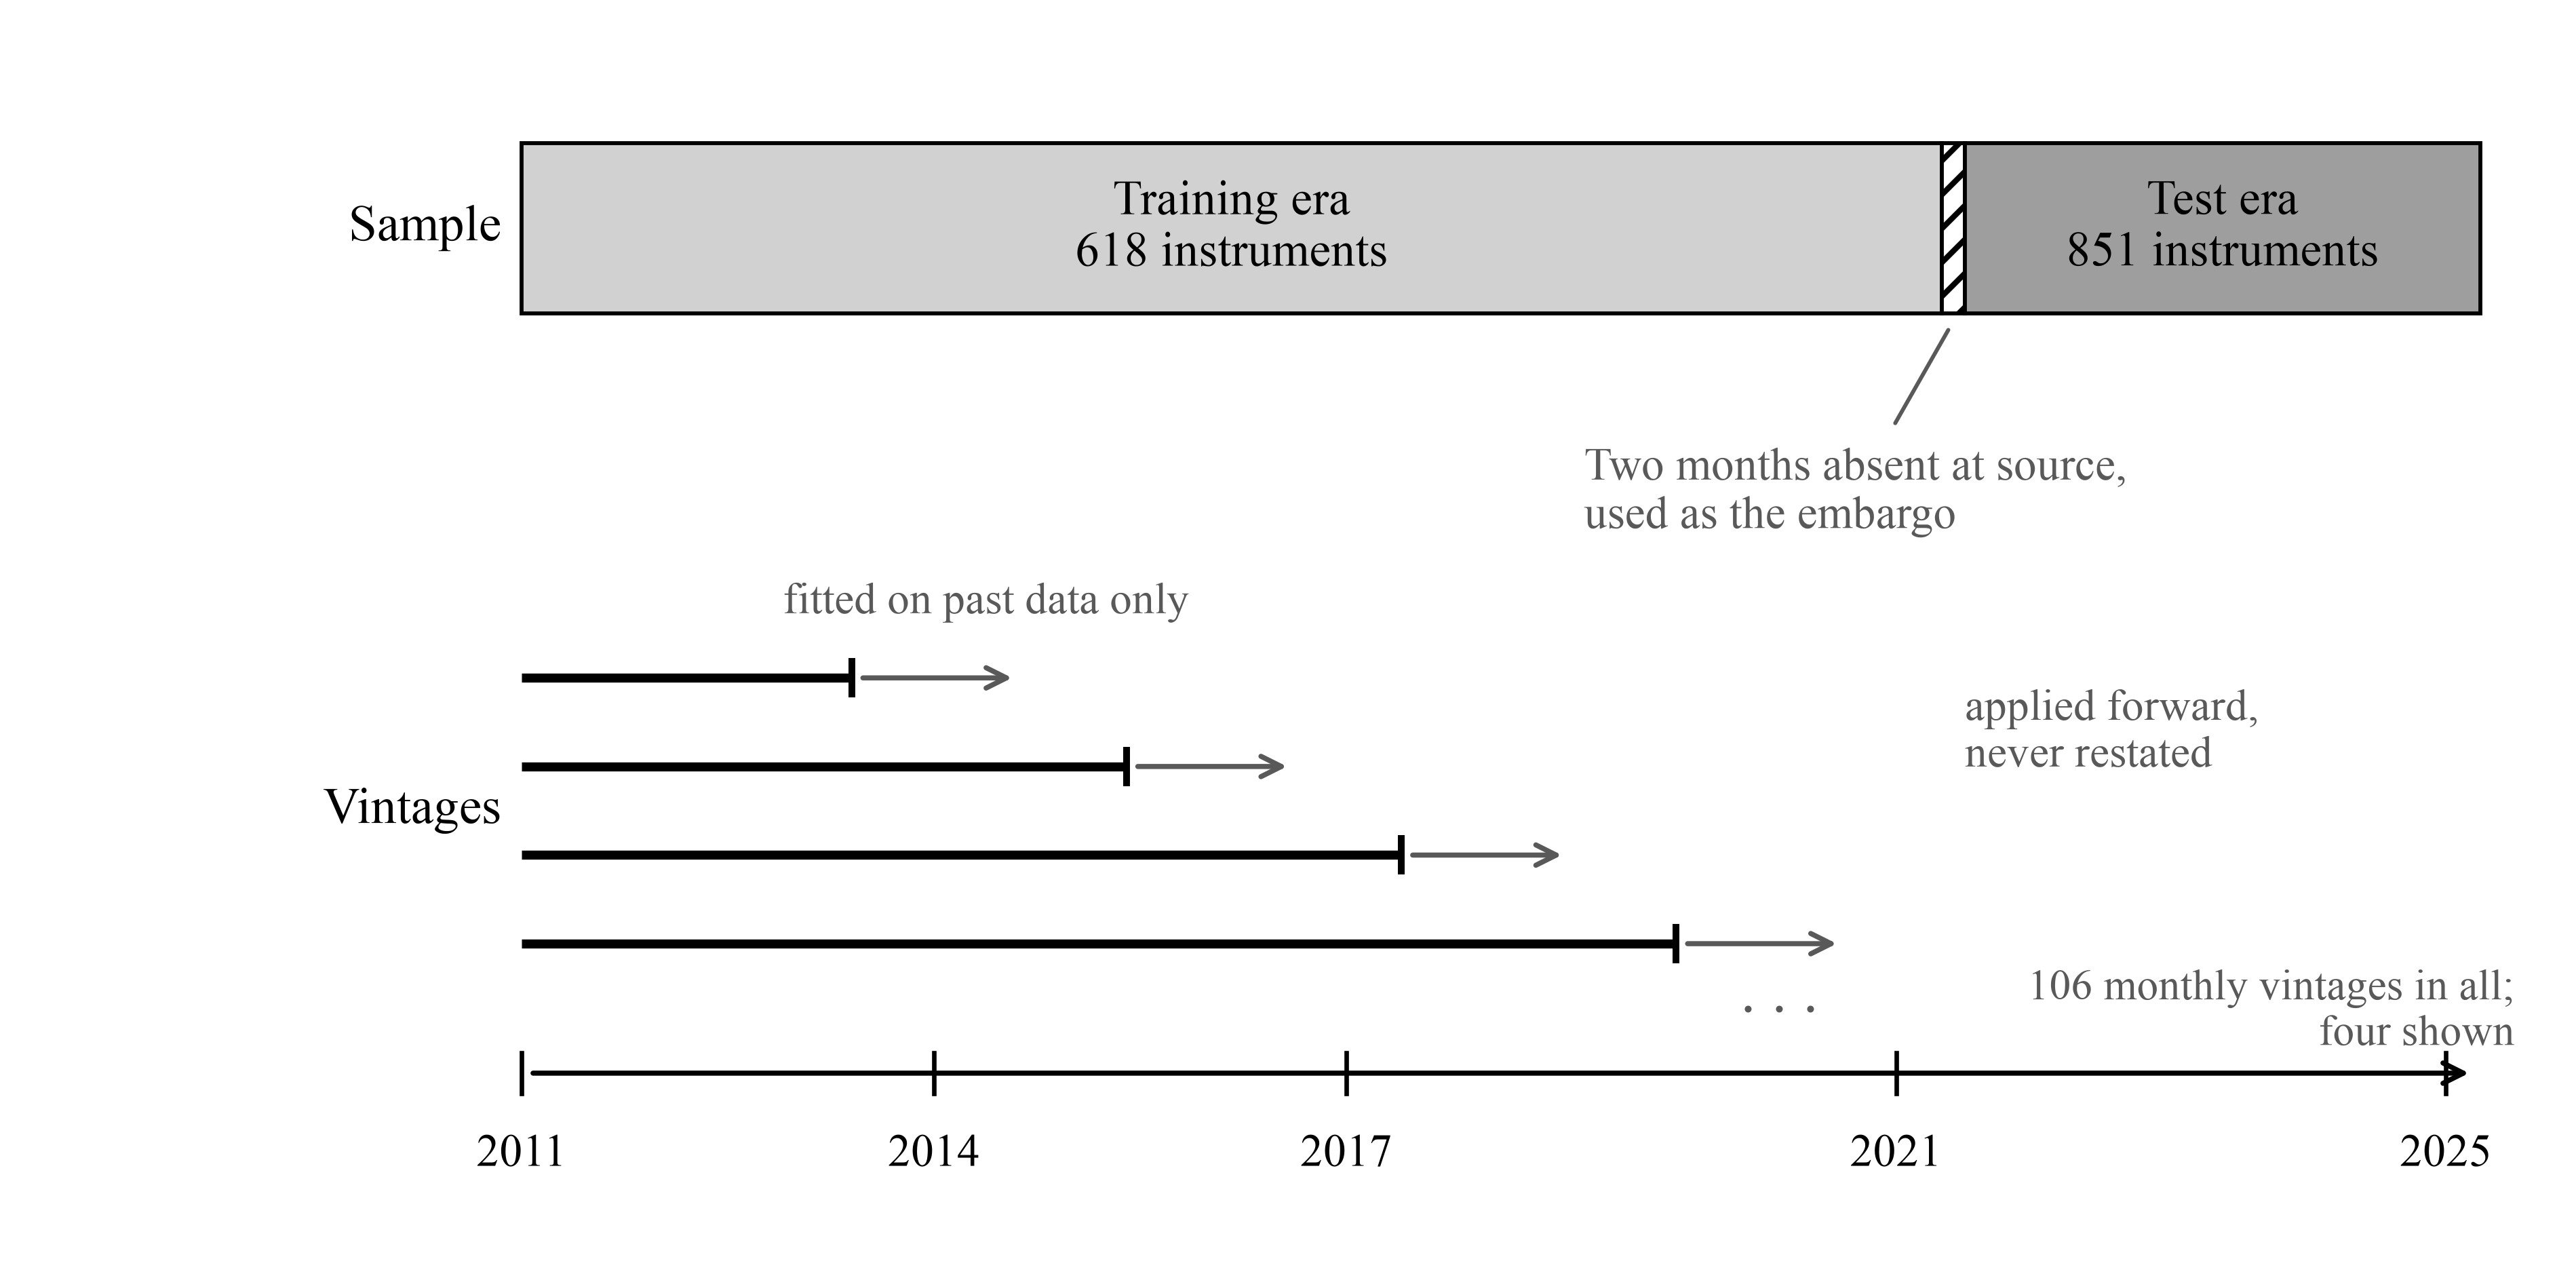
\includegraphics[width=\textwidth]{figures/figure_1_design.png}
\end{figure}

{\footnotesize\textit{Source. Authors' computation.}}

\subhead{The Regime Model and Its Hazard Layer}

Regime labels come from a three-state Gaussian hidden Markov model with diagonal covariance, fitted to four stock-day features: signed flow persistence, mean trade size against the instrument's base, and participant concentration on each side. Estimation is by expectation-maximisation on the training era alone, from one randomly located contiguous block of at most 400 days per instrument so the fit is not weighted toward recent data, with five restarts and the highest-likelihood solution retained. Ordering states on fitted persistence resolves label switching, making the naming a deterministic function of the parameters. The fitted chain is persistent: self-transition probabilities are 0.954, 0.952 and 0.978 for the buying, selling and neutral states, implying dwell times of 22, 21 and 45 days.

Parameters are then frozen and never re-estimated. Each day's state is the filtered posterior given observations to that day only, computed by the forward recursion with no smoothing pass, so no label depends on a later observation; filtered and full-sequence labels agree on 91.3\% of stock-days, and a pre-registered check confirmed the episode-level results hold on the filtered labels. An episode is a maximal run of one label, broken at calendar gaps over 21 days.

The hazard layer predicts whether an episode ends within the next \textit{k} days from episode age, the four state features, the filtered posterior, concentration drift, relative volume and log turnover. It is a gradient-boosted classifier of 200 trees at learning rate 0.05, refit once per evaluation year on episode-days ending at least ten days before that year begins.

\subhead{The Six Constraints and the Test at Each}

Each application pairs two measurements on the same object and data: what a conventional significance test reported, and what a value test reported once one constraint was imposed. An entry whose halves come from different samples is inadmissible. Decision value is defined ordinally, not monetarily: an application has decision value through constraint k if it clears constraints one to k, so the reported quantity is the index of the first constraint it fails. Two thresholds appear and differ. A screening threshold governs the regression cells establishing significance, at |t| ≥ 2.50 with a Bonferroni allowance for four cells; a gate threshold governs the forecast comparisons, at a score differential of −2.0.

Existence is assessed by panel regression. For instrument \textit{i} on day \textit{t}, with \textit{z} standardised by a past-only volatility estimate:

\begin{equation}
z^{2}_{i,t+1} \;=\; \alpha_{i} + \delta_{t} + \beta\, s_{i,t} + \boldsymbol{\gamma}'\mathbf{x}_{i,t} + \varepsilon_{i,t}
\end{equation}

where the first two right-hand terms are instrument and date fixed effects, the third is the institutional share of that instrument's turnover, and the fourth is a control vector containing log turnover. Date fixed effects absorb market-wide variation, so a market-level variable can enter only as an interaction. Standard errors are clustered on date, which accommodates arbitrary cross-sectional dependence among instruments on the same day; two-way and bootstrap alternatives are reported with the result. With samples in the hundreds of thousands, conventional significance can be readily obtained and is therefore treated as necessary rather than sufficient. Era stability uses the frozen split, with both eras reported and a sign flip counted as failure regardless of significance. Availability re-estimates equation (1) with the share taken at the lag at which it becomes knowable, holding fixed effects, controls and clustering fixed; that lag is measured from the reporting date each record carries alongside its trade date.

At market level the flow variable is constructed from the raw records as

\begin{equation}
NF_{t} \;=\; \frac{\sum_{j} b_{j,t} - \sum_{j} s_{j,t}}{G_{t-1}}
\end{equation}

where the numerator sums buy less sell value over settled equity trades on the day, and the denominator is the trailing 250-day mean of daily gross flow ending on the previous day. The pre-registered risk cell regresses next-day absolute index return on the deployable lag of that variable,

\begin{equation}
\left|r_{t+1}\right| \;=\; a + b\,NF_{t-2} + c\,NEG_{t-2} + \sum_{k=0}^{4}\varphi_{k}\left|r_{t-k}\right| + \psi\,V_{t} + u_{t}
\end{equation}

in which the second flow term is the negative part of the first and is the single permitted asymmetry, five lags of the target enter as controls alongside the implied volatility index, and standard errors are Newey-West at ten lags. Days carrying no flow observation are excluded rather than entered as zero; the alternative reading is reported alongside.

Competition scores an application against the baseline it would be deployed against rather than against zero. Three forms appear: a well-specified conditional-variance model, where the question is whether the information is already in the instrument's own history; a trivial rule capturing the same idea, compared paired on the events both act upon; and a public proxy, where the question is whether the proprietary record is needed.

Detectability asks whether the effect registers in the metric the decision consumes, which is generally not the metric that established significance. Where an application's own mechanism is the claim, this is tested by ablation: the identical machinery re-run with the mechanism removed and everything else fixed.

Execution reports the breakeven one-way cost at which net profit is zero,

\begin{equation}
c^{\ast} \;=\; \frac{\mathbb{E}\left[\pi_{t}\right]}{\mathbb{E}\left[TO_{t}\right]}
\end{equation}

the ratio of expected gross profit to expected turnover, measured in basis points per unit traded and compared against a realistic institutional cost. The breakeven is a property of the strategy; a net figure at an assumed cost is a property of the assumption, and a reader whose costs differ can use the first and cannot use the second.

\subhead{Backtest Construction and Pre-Registration}

Where a constraint requires a simulated book, a signal formed at the close of day \textit{t} is traded at the close of \textit{t + L} and earns the close-to-close return of \textit{t + L + 1}, with \textit{L} = 1. The engine is gated before use and cannot be modified without re-passing its gates: the vectorised implementation must equal a naive per-day loop; an oracle signal equal to the next day's return must produce an extreme ratio at zero lag and collapse at lag one; and a constructed book with known turnover must satisfy net equals gross less cost times turnover.

Each application's threshold was written into its stage header before its numbers existed, with the branch to be taken if it were missed. An application that misses its threshold is reported as a negative result and is not re-specified, and a gate's target is fixed with its threshold, so re-aiming a test at whichever quantity carries the effect is exploratory and labelled as such.

\subhead{Verification of Reported Figures}

Every figure clears four gates before admission. It must be fresh, the artifact no older than the code that writes it; primary, the source being the computation rather than a document describing it or a copy of its output; traced, the artifact digest matching a recorded value; and extracted, a locator identifying exactly one number reading the value back out and confirming it.

\mainhead{RESULTS AND DISCUSSION}

\subhead{Where the Applications Failed}

Figure 2 reports the attrition. Seven applications, plus one external control, are placed at the lowest constraint each fails to survive; the control is excluded from the counts and discussed separately.

\begin{figure}[htbp]
\centering
\caption{Attrition of Seven Applications Across Six Ascending Constraints}
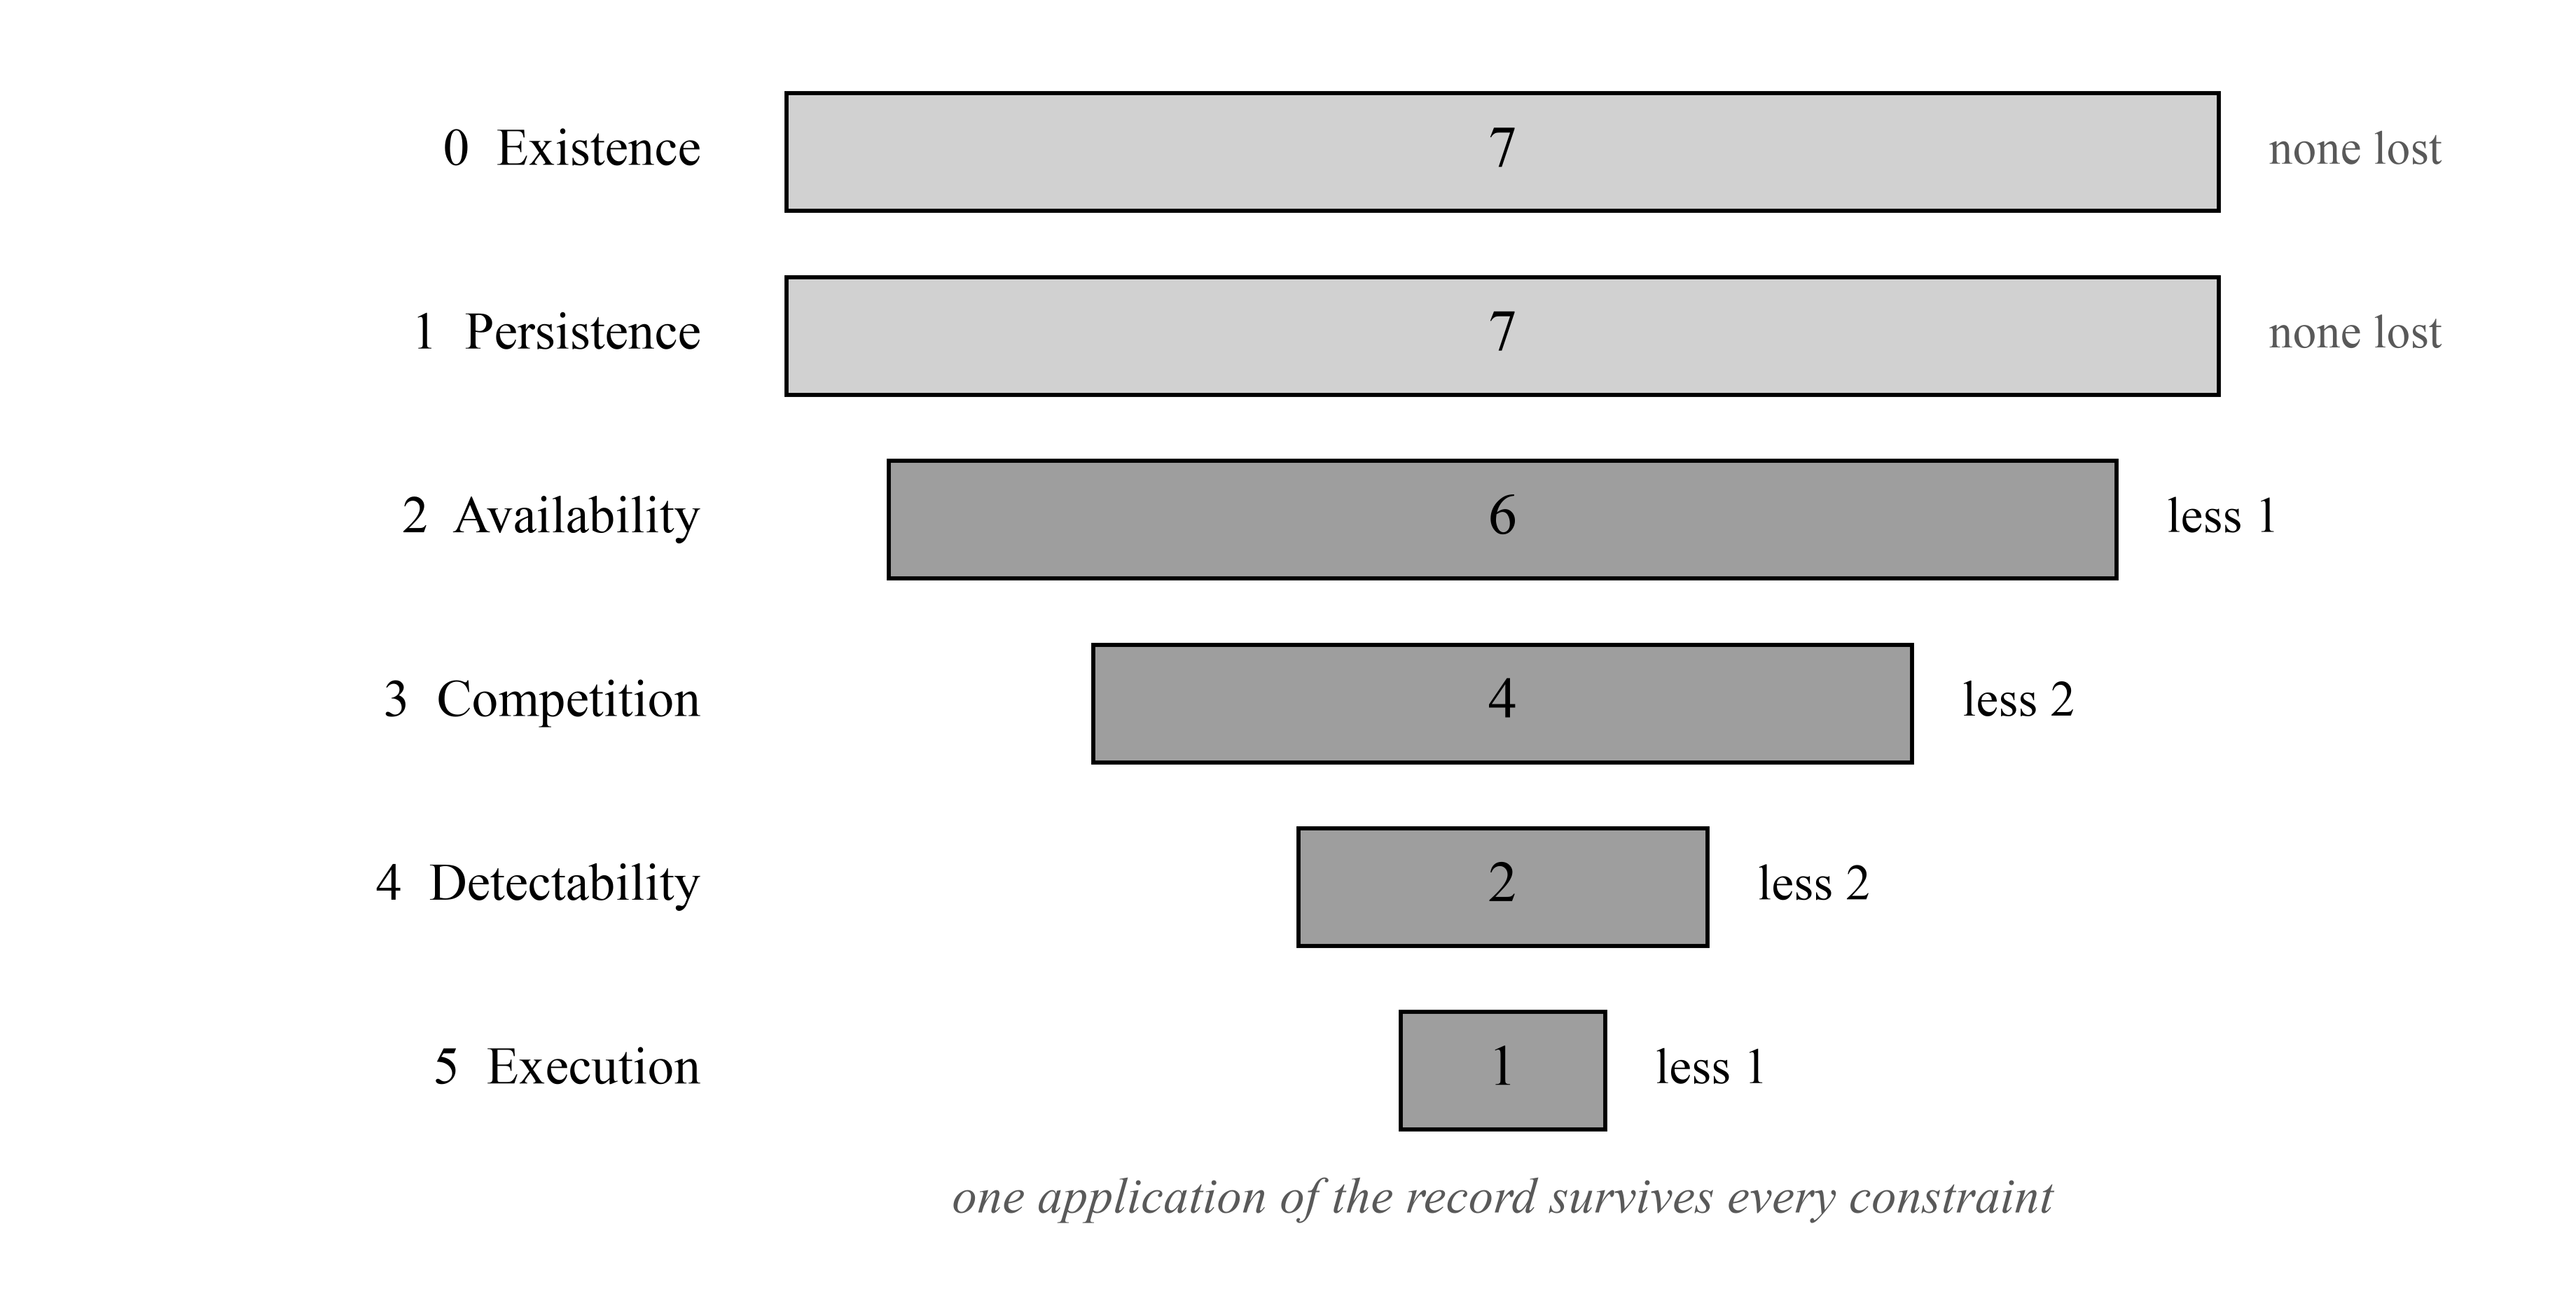
\includegraphics[width=\textwidth]{figures/figure_2_attrition.png}
\end{figure}

{\footnotesize\textit{Source. Authors' computation.}}

Nothing was lost at the first two constraints. Every application produced an effect statistically present and stable on a frozen out-of-sample era covering a substantially different cross-section, in which only 441 of the two eras' 1,028 instruments are common. This is a temporal holdout on a shifting universe, not an independent re-test, so it establishes era stability rather than replication in that literature's sense; by the weaker standard, all seven pass. Attrition began where institutional constraint did, and spread across four levels.

\subhead{Availability: Information That Arrives Too Late}

The institutional share of a stock's turnover predicts its next-day volatility. The dependent variable is the squared standardised return, so this is variation that the model's own volatility estimate has already failed to explain. Across 577,245 instrument-days, with instrument and date fixed effects and log turnover controlled, the coefficient carries \textit{t} = −5.53 in the full sample, −4.42 in training and −3.25 in test.

Every record carries the date the custodian reported it as well as the date of the trade, so the lag at which the share becomes knowable is measured from the record rather than assumed. Value-weighted over the fourteen years, 0.13\% of a day's flow is reported by that day's close, 94.30\% by the next close and 97.51\% by the second, stable across eras at 95.89\% in training and 99.27\% in test. Count-weighting gives 94.37\% and 97.30\%, and trades reported after the first day are on average 1\% larger, so the curve is not an artefact of a few large late arrivals. A two-day lag is therefore the conservative deployable choice, and the contemporaneous specification uses information of which almost none is in hand when the decision must be taken.

Taking the same predictor at that lag collapses it. Table 1 reports both specifications side by side.

\begin{table}[htbp]
\centering
\singlespacing
\caption{The Same Specification at Two Information Sets}
\begin{tabularx}{\textwidth}{>{\hsize=1.8000\hsize\RaggedRight\arraybackslash}X>{\hsize=0.7333\hsize\RaggedLeft\arraybackslash}X>{\hsize=0.7333\hsize\RaggedLeft\arraybackslash}X>{\hsize=0.7333\hsize\RaggedLeft\arraybackslash}X}
\toprule
\textbf{Information set} & \textbf{Full sample} & \textbf{Training era} & \textbf{Test era} \\
\midrule
Share known contemporaneously & −5.53 & −4.42 & −3.25 \\
Share known only at a two-day lag & −0.43 & −0.09 & −0.44 \\
\bottomrule
\end{tabularx}
\end{table}

{\footnotesize\textit{Source. Authors' computation. Entries are t-statistics on the share coefficient in equation (1), with instrument and date fixed effects, log turnover controlled and standard errors clustered on date. The contemporaneous full-sample statistic is −5.20 under two-way clustering on instrument and date, and −6.47 under a stationary date-block bootstrap; the lagged row lies between −0.42 and −0.52 under every one of these estimators.}}

Nothing differs between the rows of Table 1 except the information set: same panel, same fixed effects, same controls, same clustering. The effect does not weaken; it disappears. That places the finding as a statement about contemporaneous market structure rather than a forecast.

\subhead{Competition: The Baseline Already Holds the Information}

Two applications and the control failed here, against three different kinds of baseline.

The cleanest case is a controlled pair. Two market-level density forecasts are given the identical two-term flow tilt, the identical comparison model and the identical 2,235 scored days; they differ in one respect only, the baseline density the tilt is asked to improve. The underlying screen, equation (3) applied to the flow variable of equation (2), gives \textit{t} = −4.83 in the full sample, −2.53 in training and −2.51 in test, clearing both legs of a threshold set at |\textit{t}| ≥ 2.50 as a Bonferroni allowance for the four pre-registered cells.

\begin{table}[htbp]
\centering
\singlespacing
\caption{The Same Predictor Scored Against Two Baselines}
\begin{tabularx}{\textwidth}{>{\hsize=1.3500\hsize\RaggedRight\arraybackslash}X>{\hsize=0.8250\hsize\RaggedLeft\arraybackslash}X>{\hsize=0.8250\hsize\RaggedLeft\arraybackslash}X}
\toprule
\textbf{Measure} & \textbf{Exponentially weighted baseline} & \textbf{Asymmetric GARCH baseline} \\
\midrule
Score differential, full sample (threshold ≤ −2.0) & −2.22 (pass) & +0.28 (fail) \\
Mean score advantage ×100, training & −0.0024 & −0.0001 \\
Mean score advantage ×100, test & −0.0004 & +0.0002 (fail) \\
Coverage test probability, 5\% and 1\% levels & 0.375 and 0.248 (pass) & 0.486 and 0.248 (pass) \\
Scored days & 2,235 & 2,235 \\
\bottomrule
\end{tabularx}
\end{table}

{\footnotesize\textit{Source. Authors' computation. Both columns carry the same flow tilt and the same scored days; only the baseline volatility model differs.}}

Against the simpler baseline the tilt clears every leg. Against the better-specified one it fails both score legs and its test-era sign flips, which fails the threshold regardless of magnitude, even though its coverage is sound. Incremental value is a property of the pair, not of the predictor. Holding the evaluation window fixed changes the magnitudes but not the verdicts; scored on each engine's own longer window, the two differentials are −2.35 and −0.95.

The second case is a trivial rule. A walk-forward discrete-time hazard model forecasts whether a flow episode ends today, with yearly refits and censoring handled. Table 3 reports its skill and its decision value.

\begin{table}[htbp]
\centering
\singlespacing
\caption{Forecast Skill and Decision Value of the Episode-End Hazard Model}
\begin{tabularx}{\textwidth}{>{\hsize=1.3500\hsize\RaggedRight\arraybackslash}X>{\hsize=0.8250\hsize\RaggedLeft\arraybackslash}X>{\hsize=0.8250\hsize\RaggedLeft\arraybackslash}X}
\toprule
\textbf{Measure} & \textbf{Model} & \textbf{Age-only baseline} \\
\midrule
Area under the curve, pooled & 0.647 & 0.569 \\
Area under the curve, training & 0.637 & Not applicable \\
Area under the curve, test & 0.657 & Not applicable \\
Paired statistic on out-of-window log loss & 14.42 & Not applicable \\
Anticipation gain, test era, basis points per episode & −18 & +16 \\
Paired difference on 402 common episodes, basis points & −31 & Not applicable \\
\bottomrule
\end{tabularx}
\end{table}

{\footnotesize\textit{Source. Authors' computation.}}

The model exhibits out-of-sample discrimination under this evaluation: it beats the duration-only baseline, and better out of sample than in, which rules out memorisation. No calibration statistics are reported, and discrimination alone is not evidence that the latent mechanism is well specified. The decision layer then loses to a three-line rule on the episodes both act upon; a weaker design would have compared each against zero and declared the model the better of two positives.

Table 3 also carries a finding about the programme rather than the data. Its figures come from a re-execution on the current object; project records report an area under the curve of 0.797 and a test-era gain of +23 basis points, from a run predating an audit that rebuilt the underlying states and never re-executed afterwards. Both verdicts survive, but the discrimination is a third smaller than recorded and the decision result moved from positive to negative.

The control is a five-day foreign index return predicting next-week realised volatility of the domestic index. Its screen gives \textit{t} = −3.86, −2.91 and −4.46, among the most era-stable coefficients in the programme and stronger out of sample than in. The engine built on it fails at +1.58 against a threshold of −2.0, the positive sign meaning the tilted engine scores worse than its base. A predictor from outside the record, more era-stable than anything the record produced, failed at the same constraint by the same mechanism.

\subhead{Detectability: Effects Below the Resolution of the Metric}

Two applications survived competition and failed because the quantity a user consults cannot see them.

A participant-composition feature block produces a top-minus-bottom quintile spread of 74.8 basis points, at \textit{t} = 2.86 on non-overlapping episodes. Its incremental information coefficient over conventional flow features is 0.0012 against a threshold of 0.005, at \textit{t} = 0.67 against a bar of 2, on the same block and run. The extremes carry a spread; the average carries nothing, and the coefficient a user would consult weights the half that is empty.

The second case tests a mechanism rather than a predictor. Episode labels cluster far beyond a within-instrument shuffled null preserving each instrument's label count and destroying only temporal adjacency: mean runs of 3.61 days against 1.40 in training, 4.05 against 1.53 in test, both at \textit{p} = 0.005. The clustering holds out of sample. Table 4 reports what they contribute to the density built on them.

\begin{table}[htbp]
\centering
\singlespacing
\caption{Ablation of the Conditioning Mechanism in the Stock-Day Density}
\begin{tabularx}{\textwidth}{>{\hsize=1.8000\hsize\RaggedRight\arraybackslash}X>{\hsize=0.7333\hsize\RaggedLeft\arraybackslash}X>{\hsize=0.7333\hsize\RaggedLeft\arraybackslash}X>{\hsize=0.7333\hsize\RaggedLeft\arraybackslash}X}
\toprule
\textbf{Stratum} & \textbf{Test statistic} & \textbf{Probability} & \textbf{Score effect} \\
\midrule
Pre-registered primary stratum, uncertain label identity & −0.82 & 0.41 & −0.00004 \\
Full panel & +2.90 & 0.0037 & +0.00005 \\
\bottomrule
\end{tabularx}
\end{table}

{\footnotesize\textit{Source. Authors' computation. Positive statistics favour the conditioned system.}}

In the stratum the pre-registration nominated, where the mechanism should bind hardest, the conditioning is indistinguishable from its own removal. On the full panel it is statistically favoured, by five parts in a hundred thousand of a score whose level is about 0.55, roughly one part in eleven thousand. Comparison against an external benchmark establishes that a system is better; only ablation establishes why, and the answer here is the empirical shape of the standardised distribution rather than the flow record the system is named for.

\subhead{Execution: The Edge and Its Cost Are the Same Order}

A mechanical long-short book on the concentration measure records a gross ratio of 1.36 in training and 1.51 in test. It carries no fitted model, so what is priced is the data rather than an architecture.

Its breakeven one-way cost, from equation (4), is 7.33 basis points in training and 7.41 in test. Against an assumed 15 basis points — a round figure used throughout this programme as the centre of a 0-to-30 grid, not an estimate of any desk's costs — the breakeven is roughly half, and at that cost the book records −1.42 and −1.53. The breakeven is a property of the strategy; the net ratio is a property of the cost assumption. Neither prices capacity, borrow or market impact. The edge and the cost of capturing it are the same order, and the cost is larger.

\subhead{What Survived}

One application cleared every constraint: the record aggregated to market level, entering a Student-t density at a two-day reporting lag against a baseline that does not already contain it, as reported in the first column of Table 2. Its conditions are the ones the six failures violate: aggregation to a level where the measurement is stable, availability at a deployable lag, a magnitude the consuming metric can resolve, and a baseline that has not already absorbed it.

The survivor's role is to show that attrition is not universal, which makes the sequence a boundary rather than a verdict. That role needs one demonstrated case, not a confirmed general effect, and the pass is reported on those terms, conditional in four ways. It holds against a comparison model carrying implied volatility; scored against the bare exponentially weighted baseline, the same tilt gives −1.29 and misses its own threshold. It holds on its own evaluation window, where a one-sided probability of 0.0095 becomes 0.038 under a Bonferroni or Holm correction across the four engine gates, against 0.052 on the window common to the two market-level engines. It holds under a correction treating those four gates as a fixed family when they were a sequential search: each threshold was fixed before its own run, but the second was written after the first had passed, so the adjustment understates the search cost. And it holds under a score integrated across the 1st to 99th percentiles and weighted toward the centre, which establishes an improvement in the specified predictive density rather than in the far-tail estimate a risk manager consumes. One point runs the other way: of the four engines, only this one was left unchanged by two later estimation corrections that widened its siblings from narrow misses into clear failures. The surviving result is this aggregation, at this lag, against this baseline, on this window, under this score, and it is offered as a demonstrated possibility rather than an exploitable edge.

\mainhead{MANAGERIAL AND PRACTICAL IMPLICATIONS}

Six applications of one record failed at four different constraints. They differ in aggregation, target, horizon, estimator, baseline and metric at once, so the design cannot isolate use as the cause; what it shows is that different implementations of one record meet different binding constraints. No sentence about whether this data carries information is well posed without naming the implementation.

\textit{Establish the Binding Constraint Before Establishing Significance.} The significance question was answered affirmatively for all seven applications and settled nothing. A regression re-run at a deployable lag, a better-specified baseline, a trivial rule paired on shared events, and an ablation each cost little beyond machinery already written, and each removed an application no additional data or model capacity would have touched.

\textit{Name the Baseline, Not the Benchmark.} A vendor evaluation that scores a dataset against a weak alternative is measuring the alternative. Table 2 shows the same tilt passing against one baseline and failing against another, nothing about the data changed. Buyers should specify the production baseline the dataset must improve, and treat a demonstration against anything weaker as uninformative.

\textit{Aggregate to Where the Measurement Is Stable.} The single surviving use is the most aggregated one: the stock-day applications failed at availability, detectability and cost, while the market-level application cleared every constraint. This is consistent with the identifier constraint documented above, and suggests that the frequency at which an alternative dataset is reported need not be the frequency at which it is informative.

\textit{Implications for the Indian Market.} Three readings apply here. The surviving application is a market-level risk forecast, where a domestic risk manager or an exchange monitoring aggregate exposure would use it, not a stock-selection input. The stock-day results place foreign institutional composition as contemporaneous market structure rather than forecast, consistent with the informational-disadvantage reading Raizada and Nawn (2025) report here. And the breakeven costs of 7.33 and 7.41 basis points sit below plausible execution costs here, so the concentration measure is usable only by an agent whose trading costs are already committed. As Maheshwari and Naik (2026) document a shift from foreign to domestic institutional dominance in this market, the aggregate flow variable that survived here should be re-estimated on domestic institutional flow before it is relied upon in future periods.

For risk practice, the ablation in Table 4 carries a further implication. A model that beats an external benchmark has established that it is better, not why. Where a system is named for a conditioning mechanism, that mechanism should be ablated and the effect size reported: routine in machine learning, and close to absent from risk-model validation.

\mainhead{CONCLUSION}

A fourteen-year record of foreign institutional flow was applied at seven points in a modelling stack under six ascending constraints. Every application cleared its own prespecified significance threshold and held on a frozen out-of-sample era covering a substantially different cross-section. Six then failed to reach a use.

One failed because the effect was not knowable at the lag a decision requires. Two failed because the baseline they would improve already contained the information, one of them the same predictor that passes against a simpler baseline, which shows incremental value is a property of the pair rather than of the data. Two failed because the effect lay below the resolution of the metric a user would consult, one of them the conditioning mechanism the system is named for. One failed because its breakeven cost of 7.41 basis points is roughly half the assumed cost.

One survived, under conditions the six failures violate, as a demonstrated possibility rather than an exploitable edge. A control predictor from outside the dataset, more era-stable than anything the record produced, failed at the same constraint by the same mechanism, consistent with the difficulty arising in the transition from statistical evidence to institutional use rather than in this data.

Applying the verification protocol to the source programme also located a metrics table quoted from a stale copy, two pre-registered gating regressions with no producing stage, and one stage whose reported effect size was a third larger than its current object supports. None changed a verdict; all changed a figure that had already been written down.

\mainhead{LIMITATIONS OF THE STUDY AND SCOPE FOR FURTHER RESEARCH}

The ordering is argued from logical dependence, since a failure at a lower constraint invalidates those above it. The distribution of failures across constraints is a fact about seven applications of one record in one market, and nothing here establishes that it generalises. A single external control shows the attrition is not peculiar to flow data, but cannot establish its shape in general.

The six constraints span the deployment stages these applications encountered, and are not claimed exhaustive: regulatory limits, capacity and post-publication decay of the kind Pénasse (2022) models were not imposed. Availability and execution rest on one application each, an illustration rather than a distribution.

Three instruments the framework identifies were not applied, each carrying a different exposure.

The episode design has heterogeneous treatment timing, the setting in which two-way fixed effects is biased, and the corrections compared by Aguilar-Loyo (2025) and developed by de Chaisemartin and D'Haultfœuille (2026) were not used; the direction of that bias cannot be signed in advance. The exposure is bounded: episode-level estimation enters only the application in Table 4, so the surviving result is unaffected.

Eight strategy books were also examined, of the kind of search Arian et al. (2024) evaluate, and are not priced; none passed, so no positive claim rests on them. The engine search is priced above, with the caveat that the family was sequential rather than fixed.

Expected shortfall was assessed through a coverage ratio rather than a test, so a direct backtest could reject where the ratio appeared satisfactory. The tail-calibration framework of Allen et al. (2025) or the decompositions of Arnold et al. (2024) could move the density comparison either way, which is why the surviving claim is stated above as holding under the score used rather than in the far tail.

Closing these is the natural extension of this work.

The underlying transaction data is proprietary. Derived artifacts are retained, and every reported figure is bound to an artifact, a locator within it and a recorded digest, so a reader with access can check any figure without reading the analysis code, though that access is not general. Reproducibility is machine-local: every figure regenerates from a recorded command, establishing that the numbers descend from computations the authors ran, not that another environment would reproduce them exactly.

\mainhead{Author's Contribution}

The author conceived the research design, assembled and validated the dataset, implemented the modelling stack and the verification protocol, conducted all analyses, and wrote the manuscript.

\mainhead{Conflict of Interest}

The author certifies that there is no conflict of interest with any financial or non-financial interest in the subject matter discussed in this manuscript.

\mainhead{Funding Acknowledgement}

The author received no financial support for the research, authorship, or publication of this article.

\mainhead{REFERENCES}

Aguilar-Loyo, J. (2025). A comparative analysis of two-way fixed effects estimators in staggered treatment designs. Journal of Econometrics, 251, 106059. https://doi.org/10.1016/j.jeconom.2025.106059

Allen, S., Koh, J., Segers, J., \& Ziegel, J. (2025). Tail Calibration of Probabilistic Forecasts. Journal of the American Statistical Association, 120(552), 2796-2808. https://doi.org/10.1080/01621459.2025.2506194

Arian, H., Norouzi Mobarekeh, D., \& Seco, L. (2024). Backtest overfitting in the machine learning era: A comparison of out-of-sample testing methods in a synthetic controlled environment. Knowledge-Based Systems, 305, 112477. https://doi.org/10.1016/j.knosys.2024.112477

Arnold, S., Walz, E. M., Ziegel, J., \& Gneiting, T. (2024). Decompositions of the mean continuous ranked probability score. Electronic Journal of Statistics, 18(2). https://doi.org/10.1214/24-ejs2316

Azevedo, V., Kaiser, G. S., \& Mueller, S. (2023). Stock market anomalies and machine learning across the globe. Journal of Asset Management, 24(5), 419-441. https://doi.org/10.1057/s41260-023-00318-z

Bagnara, M. (2024). Asset Pricing and Machine Learning: A critical review. Journal of Economic Surveys, 38(1), 27-56. https://doi.org/10.1111/joes.12532

Bowles, B., Reed, A. V., Ringgenberg, M. C., \& Thornock, J. R. (2024). Anomaly Time. The Journal of Finance, 79(5), 3543-3579. https://doi.org/10.1111/jofi.13372

Chai, D., Ali, S., Brosnan, M., \& Hasso, T. (2026). Understanding researchers' perceptions and experiences in finance research replication studies: A pre-registered study. Pacific-Basin Finance Journal, 96, 103061. https://doi.org/10.1016/j.pacfin.2026.103061

Chopra, F., Haaland, I., Roth, C., \& Stegmann, A. (2023). The Null Result Penalty. The Economic Journal, 134(657), 193-219. https://doi.org/10.1093/ej/uead060

Coyle, D., \& Manley, A. (2024). What is the value of data? A review of empirical methods. Journal of Economic Surveys, 38(4), 1317-1337. https://doi.org/10.1111/joes.12585

de Chaisemartin, C., \& D’Haultfœuille, X. (2026). Difference-in-Differences Estimators of Intertemporal Treatment Effects. Review of Economics and Statistics, 108(4), 863-880. https://doi.org/10.1162/rest\_a\_01414

Dey, M., Mishra, S., \& De, S. (2024). A Study on How Institutional Investors Respond to Risk, Return and Volatility: Evidence from the Indian Stock Market. Journal of the Knowledge Economy, 15(1), 5072-5093. https://doi.org/10.1007/s13132-023-01718-7

Ding, Y., Kambouroudis, D., \& McMillan, D. G. (2025). Forecasting realised volatility using regime-switching models. International Review of Economics \& Finance, 101, 104171. https://doi.org/10.1016/j.iref.2025.104171

Ghachem, M., \& Ersan, O. (2025). Estimation of the probability of informed trading models via an expectation-conditional maximization algorithm. Financial Innovation, 11(1). https://doi.org/10.1186/s40854-024-00729-w

Gonçalves, S., McCracken, M. W., \& Yao, Y. (2025). Bootstrapping out-of-sample predictability tests with real-time data. Journal of Econometrics, 247, 105916. https://doi.org/10.1016/j.jeconom.2024.105916

Hou, K., Xue, C., \& Zhang, L. (2020). Replicating Anomalies. The Review of Financial Studies, 33(5), 2019-2133. https://doi.org/10.1093/rfs/hhy131

Jensen, T. I., Kelly, B., \& Pedersen, L. H. (2023). Is There a Replication Crisis in Finance? The Journal of Finance, 78(5), 2465-2518. https://doi.org/10.1111/jofi.13249

Kaplanski, G. (2023). The race to exploit anomalies and the cost of slow trading. Journal of Financial Markets, 62, 100754. https://doi.org/10.1016/j.finmar.2022.100754

Li, Z., Liu, L. X., Liu, X., \& John Wei, K. C. (2024). Replicating and Digesting Anomalies in the Chinese A-Share Market. Management Science, 70(8), 5066-5090. https://doi.org/10.1287/mnsc.2023.4904

Maheshwari, S., \& Naik, D. R. (2026). From FII Dependence to DII Dominance: Behavioral Dynamics and Minskyan Risk in India’s Stock Market. Journal of Risk and Financial Management, 19(5), 315. https://doi.org/10.3390/jrfm19050315

Muravyev, D., Pearson, N. D., \& Pollet, J. M. (2025). Anomalies and Their Short-Sale Costs. The Journal of Finance, 80(6), 3639-3694. https://doi.org/10.1111/jofi.13501

Pénasse, J. (2022). Understanding Alpha Decay. Management Science, 68(5), 3966-3973. https://doi.org/10.1287/mnsc.2022.4353

Raizada, G., \& Nawn, S. (2025). Trade informativeness of foreign investors in India. Journal of Asset Management, 26(1), 83-90. https://doi.org/10.1057/s41260-024-00387-8

Sak, H., Huang, T., \& Chng, M. T. (2024). Exploring the factor zoo with a machine-learning portfolio. International Review of Financial Analysis, 96, 103599. https://doi.org/10.1016/j.irfa.2024.103599

Sun, Y., Liu, L., Xu, Y., Zeng, X., Shi, Y., Hu, H., Jiang, J., \& Abraham, A. (2024). Alternative data in finance and business: emerging applications and theory analysis (review). Financial Innovation, 10(1). https://doi.org/10.1186/s40854-024-00652-0

Thapa, C., Neupane, B., Shrestha, C., \& Bhattarai, N. P. (2026). Policy information uncertainty and foreign institutional investors trading behavior: evidence from India. Review of Quantitative Finance and Accounting, 67(1), 45-79. https://doi.org/10.1007/s11156-025-01448-8

Waghmare, K., \& Ziegel, J. (2026). Proper Scoring Rules for Estimation and Forecast Evaluation. Annual Review of Statistics and Its Application, 13(1), 271-296. https://doi.org/10.1146/annurev-statistics-042424-050626

\end{document}
